\chapter{Mission Principale}
Ma mission lors de cette 5ième année a été de continuer le développement de l'application mobile Callibri Mobile
que j'ai commencé vers le milieu de la 4ième année, cette application est la refonte complète de l'ancienne 
application mobile qui n'est qu'un wrapper de navigateur autour du site web2 en responsive,
aujourd'hui les application mobiles étant un passage obligatoire pour fournir aux clients une experience 
correcte d'utilisation de nos services et pour rester compétitif face à nos concurrent 
il était nécéssaire de réaliser une application qui soit pensé pour une interface de smartphone et 
non juste une adaptation. \newline

lors de la 4ième année je me suis familiarisé avec Ionic et Angular, les deux framework que j'ai utilisé pour 
le développement de l'application, Ionic est un framework qui permet de créer des application mobile 
iOS et Android mais aussi desktop via electron en utilisant des technologies web.\newline

Au début du développement Ionic n'était qu'à ses balbutiements avec la version 1.3 et utilisait uniquement 
le framework angular, j'ai du très tôt dans le cycle de déveleppement porter la version vers ionic 2 qui n'etait pas retro 
compatible.\newline

Lors de ma 5ième année Ionic a subis de nombreux changements, le plus notable étant le changement de la version 3 
à la version 4, ce dernier est devenu framework-agnostic c'est à dire qu'il ne dépend plus d'un framework 
web sousdjacent spécifique mais peut être utilisé par les autres framework web les plus connus tel que 
React et vuejs mais aussi en standalone avec du javascript pure. \newline 

Comme nous avant passé plus d'un an à développer l'application en utilisant le framework Angular nous 
avons décider de continuer ce qui n'a pas empecher le fait que le changement de version 
a entrainé de nombreux changement qui fut le but principal de ma mission de 5ieme année. \newline

En passant à sa version 4, Ionic apporte grand nombre de changement:

\begin{itemize}
	\item passage d'angular 2+ à angular 7+: un grand bon en avant en terme de performance, ce qui 
	est très rechercher pour le développement hybride d'application mobile car cela permet de reduire 
	la différence de fluidité avec une application native. \newline

	\item utilisation du router angular en lieu et place du navcontroller de ionic:
	l'équipe de développement de Ionic à decider de permettre d'utiliser le meilleur 
	de chaquer framework du stack et le routeur angular en fait partie, cela fut une 
	partie assez difficile à mettre correctement en place car l'application 
	callibri mobile à une grande quantité de page et de modales. \newline 

	\item apparition du shadow-dom: un nouveau système utilisé dans le rendu du DOM,
	le shadow DOM est comme un subtree du DOM, il permet notammenet de simplifier 
	le fonctionnement des règles CSS mais surtout d'augmenter les performance de rendu 
	de l'html qui sont loin d'être optimales dans le cas d'un smartphone. \newline
	\begin{figure}[!h]
		\centering
		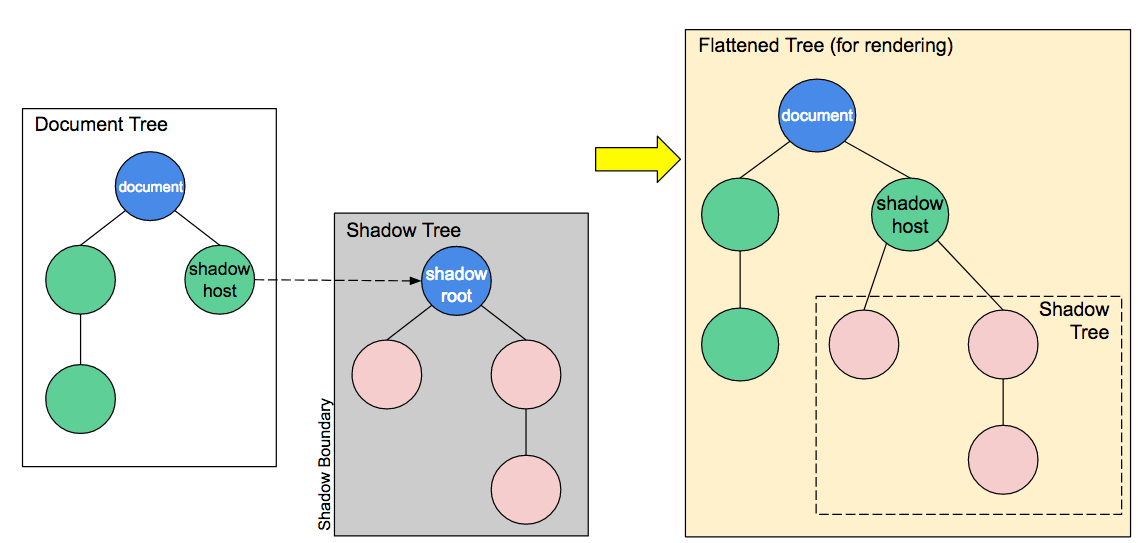
\includegraphics[width=1\linewidth]{Images/shadow}
		\caption{fonctionnement du shadow dom}
		\label{fig:archhexa}
	\end{figure}

	\item De nombreux changement dans le fonctionnement des composants Ionic et de leur 
	syntax ce qui a du nécéssiter la réecriture d'une bonne partie des fichiers html 
	de l'application plus un changement de l'architecture des fichiers du projet 
	pour refleter ces divers changement. \newline
\end{itemize}

Tout ces changments ont aussi été l'occasion de perfectionner le look de l'application 
et l'intuitivité de ses interfaces, le fastmenu qui etait un menu d'accès rapide sous 
forme de cercle disponible sur toutes les pages de l'application a été supprimé,
il prenait beaucoup de place inutilement pour être une duplication des contrôles 
déjà disponibles. \newline 

\section{Agenda}
Ce fut la partie de l'application qui a subis le plus de changement, anciennement l'agenda 
utilisait du code de très mauvaise qualité pour répondre à un besoin technique presque inexistant.
l'agenda utilise deux vues: la vue jour et la vue mois, dans l'ancienne version majeure
de l'application un système de cache complexe était utilisé pour charger une semaine entière 
et ainsi ne pas avoir à faire des appel regulier au serveur, pour l'affichage 
un système de slide tout aussi complexe était utilisé pour faire correspondre le jour affiché 
avec un des 7 jours en cache, cet ensemble était très mal écrit, tout à fait intestable 
et peu performant.

pendant ma 5ième année j'ai refait cette page agenda, qui est la page la plus importante 
de tout l'application, en supprimant ce système de cache qui était plus source d'erreur 
et de difficulté de maintenabilité qu'autre chose puisqu'au final la requête pour charger 
un jour de l'agenda depuis le serveur est très simple et rapide.


\newpage
\section{Bilan et recul sur la mission}
Pour cette mission j'ai eu totale liberté dans mes choix qui fut à la fois un avantage mais 
aussi une preuve du manque de gestion de projet au sein de l'entreprise, je n'avais 
aucun cahier des charges et les règles métiers n'etaient pas clairement définies,
j'ai du donc établir par moi même le cahier des charge et lister les nouvelles fonctionnalitées 
en me basant sur l'ancien site web et son code qui n'a d'ailleurs pas facilité la tache. \newline

j'ai du aussi me baser sur le website et m'auto-former aux bonnes pratiques 
à appliquer à l'expérience utilisateur et l'interface graphique puisqu'une application
n'a pas du tout les mêmes contraintes qu'un site web. \newline

En prenant du recul je me suis rendu que le choix du framework Ionic était un choix judicieux 
mais seulement à court terme, il est en effet assez difficile de maintenir toute 
application basé sur le javascript et l'environement node car les outils et la qualité 
d'un environement de déveleppement basé sur ces techno est assez médiocre, les librairie 
deviennent incompatibles ou non d'une version sur l'autre, il est assez difficile 
de débugger certaines erreurs à cause de l'epaisseur conséquente du stack de technologies
utilisées. Si je n'avais pas eu d'aussi forte contraintes de temp pour produire un résultat 
j'aurais utilisé le framework Xamarin qui aurait encore plus augmenté la portabilité 
du code puisque j'aurais pu utiliser le noyau métier du web3 dans l'application
ce qui aurait permis de réduire le temp de développement et peut être arriver 
à produire un résultat aussi rapidement qu'avec l'utilisation du framework Ionic, 
au moment des choix technologique j'ai peut être donc fait preuve d'un manque de vision génerale
et sur le long terme. \newline


